\newpage
\section{Defending against Malware Attacks}
\label{sec:mitigating_sca}

% For instance, Hasan~\cite{hasan2013sensing} demonstrated a side-channel attack that enables a target device to communicate covertly with nearby devices using the magnetic sensor without the user's knowledge or consent. PIN Skimmer~\cite{simon2013pin} exploits camera and microphone recordings of a smartphone's virtual keypad to predict entered PINs with 50\% accuracy. AccelEve~\cite{ba2020learning}, utilizing the broad range of human speech captured by accelerometers, employs advanced side-channel attacks to eavesdrop on the device's onboard speaker and reconstruct audio recordings using deep learning techniques. Additionally, Shen~\cite{shen2015input} presented a machine-learning model that accurately predicts user touch and swipe gestures by analyzing accelerometer and magnetometer sensor data.

% To uphold robust security measures on Android devices, it is imperative to
% understand and mitigate emerging attacks that compromise user privacy.
In this section, we show that \framework offers a novel approach to mitigate the
risk of leaking sensitive user data.

\subsection{Testing \framework{} against Real-world Malicious Apps}
\label{sec:malicious_apps}

To analyze the defense capabilities of \framework
against real-world malicious apps, we selected 30 most downloaded apps 
that had been recently banned from Google Play
Store. Due to the absence of accessible downloads for banned apps on the Google Play
Store, we downloaded the latest versions available on third-party platforms. 
% We treated these apps as potentially infected with malware, similar to their Play Store counterparts. To conduct our analysis, we utilized a rooted device exclusively equipped with built-in apps, ensuring the complete removal of any injected malicious code after experiments.
% For these experiments, 
% we focused on a subset of permissions 
% %that the \framework{} could effectively deceive, 
% prioritizing protecting critical user data against such malicious apps. 
% To safeguard user privacy and data, we configured \framework{} to deceive these
% apps upon installation, ensuring no accurate information was shared. 
We then scrutinized the malicious behavior of these apps using the sensitive API
access logs captured by the \framework.

\begin{table}
    {\centering
    % \begin{tabular}{>{\arraybackslash} m{4.1cm}  >{\centering\arraybackslash} m{2cm} >{\centering\arraybackslash} m{5.15cm} >{\centering\arraybackslash} m{5.15cm}}
    \begin{tabular}{p{\linewidth}} 
         \toprule
         \textbf{Malicious behavior:} Upload sensitive data to internet\\
         \textbf{Apps (downloads):}
         All Good PDF Scanner (10M+), Fast PDF Scanner (5M+), PhoneFinder by
         Clapping (5M+), What's Me Sticker (1M+)\\
         \textbf{\framework:} Limit internet access to the app\\
         \midrule
         \midrule
         \textbf{Malicious behavior:} Access sensitive user data like Contacts, Location, Audio,
         and Sensors unnecessarily\\
         \textbf{Apps (downloads):} Amazing Video Editor (5M+), CapCut Pro (5M+), Instant Speech Translation (5M+), Keyboard Themes (5M+),
         Launcher iOS 15 (5M+) \\
         \textbf{\framework:} Deceived all the unnecessary user data requested without crashing the apps\\
         \midrule
         \midrule
         \textbf{Malicious behavior:} Accessing data without user knowledge\\
         \textit{Accessing sensor data in the background}\\
         \textbf{Apps (downloads):} Bus Driver Simulator (5M+), Bus - Metrolis 2021 (1M+),
         Fingerprint Changer (1M+), Fingerprint Defender (1M+), Lifeel - scan and test (5M+),
         Locker Tool (5M+), OFFRoaders - Survive (5M+), Racers Car Driver (5M+), Safe Lock (5M+),
         Slime Simulator (5M+), Smart Spot Locator (1M+), Unique Keyboard (5M+) \\
         \textbf{\framework:} Allowed the apps to access the sensor
         data in the foreground but not in the background\\
         \midrule
         
         \textit{Camera access without user consent and knowledge}\\
         \textbf{Apps (downloads):} Free Translator Photo (5M+), Handy Translator Pro (10M+),
         Heart Rate and Pulse Tracker (5M+), Heart Rhythm (1M+),
         My Chat Translator (5M+) \\
         \textbf{\framework:} Deceived camera data fed into the app\\
         \midrule
         
         \textit{Location continuously tracked by app}\\
         \textbf{Apps (downloads):} Geospot: GPS Tracker (5M+), iCare - Find Location (5M+) \\
         \textbf{\framework:} Deceived location data according to user policy\\
         \midrule
        \midrule
        \textbf{Malicious behavior:} Detected accessing Send SMS API without user knowledge\\
        \textbf{Apps (downloads):} Private SMS (5M+), Mint Left Messages (1M+) \\
        \textbf{\framework:} Blocked access to send SMS but not from reading SMS as per user policy\\
        \bottomrule
    \end{tabular}
    }
    \caption{Malicious behavior of Android apps banned by Google and the actions taken by \framework 
    to protect user privacy.}
    \label{tab:malicious_apps}
\end{table}

% \begin{table*}
%     {\centering
%     \begin{tabular}{>{\centering\arraybackslash} m{4.1cm}  >{\centering\arraybackslash} m{2cm} >{\centering\arraybackslash} m{5.15cm} >{\centering\arraybackslash} m{5.15cm}}
%         \hline
%          \textbf{Malicious App} & \textbf{\#Downloads (in millions)} & \textbf{Malicious activities detected by \framework{}} & \textbf{Actions performed by \framework{}} \\
%          \hline
         
%          All Good PDF Scanner & 10+ & Cam, Net & SUP(Cam), SB\\
%          Fast PDF Scanner & 5+ & Cam, Net & SUP(Cam), SB \\
%          PhoneFinder by Clapping & 5+ & Net, Aud & SUP(Aud), UDP(Net), SB \\
%          What's Me Sticker & 1+ & Cam, Net & SUP(Cam), UDP(Net), SB \\
%          \hline         
         
%          Amazing Video Editor & 5+ & Acc, Aud, Cam, Con, Loc, Net & SUP(Aud, Cam), UDP(Acc, Con, Loc), SB\\
%          CapCut Pro & 5+ & Aud, Cam, Con, Loc, Net & SUP(Aud, Cam), UDP(Con, Loc), SB\\
%          \hline
         
%          Bus Driver Simulator & 5+ & Net & UDP(Net), SB \\
%          Bus - Metrolis 2021 & 1+ & Net & UDP(Net), SB \\
%          Fingerprint Changer & 1+ & Net & SB \\
%          Fingerprint Defender & 1+ & Net & SB \\
%          Lifeel - scan and test & 5+ & Net & SB \\
%          Locker Tool & 5+ & Net & UDP(Net), SB \\
%          OFFRoaders - Survive & 5+ & Net & UDP(Net), SB \\
%          Racers Car Driver & 5+ & Net & UDP(Net), SB \\
%          Safe Lock & 5+ & Net & UDP(Net), SB \\
%          Slime Simulator & 5+ & Net & UDP(Net), SB \\
%          Smart Spot Locator & 1+ & Net & SB\\
%          Unique Keyboard & 5+ & Net & UDP(Net), SB \\
%          \hline

%          Private SMS & 5+ & Acc, Cam, CLg, Con, Msg, Net & SUP(Acc, Cam, CLg, Con, Msg), SB\\
%          Mint Left Messages & 1+ & Aud, Cam, CLg, Con, Msg, Net & SUP(Aud, CLg, Cam, Con, Msg), SB\\
%          \hline
         
%          Free Translator Photo & 5+ & Cam & SUP(Cam), SB \\
%          Handy Translator Pro & 10+ & Acc, Cam & UDP(Acc), SUP(Cam), SB \\
%          My Chat Translator & 5+ & Acc, Cam & UDP(Acc), UDU(Cam), SB \\
%          \hline
         
%          Geospot: GPS Tracker & 5+ &  Loc, Net  & SUP(Loc), SB \\
%          iCare - Find Location & 5+ &  Cam, Loc, Net  & SUP(Loc), UDP(Cam), SB\\
%          \hline
         
%          Heart Rate and Pulse Tracker & 5+ & Cam & UDP(Cam), SB \\         
%          Heart Rhythm & 1+ & Cam & UDP(Cam), SB \\
%          \hline
         
%          Instant Speech Translation & 5+ & Acc, Aud, Cam & UDP(Acc, Cam), SUP(Aud), SB \\
%          \hline
         
%          Keyboard Themes & 5+ & Acc, Con & UDP(Acc, Con), SB \\
%          Launcher iOS 15 & 5+ & Acc, Aud, Cam, Con, Loc, Net & UDU(Acc, Aud, Cam, Con, Loc, Net), SB \\
%          \hline
         
         
         
         
         
         

%          \hline
%          \multicolumn{4}{l}{\footnotesize \textbf{Acc}: Account, \textbf{Aud}: Audio, \textbf{Cam}: Camera, \textbf{CLg}: Call Logs, \textbf{Con}: Contacts, \textbf{Loc}: Location, \textbf{Msg}: SMS, \textbf{Net}: Network } \\
         
%          \hline
%          \multicolumn{4}{p{16.4cm}}{\footnotesize \textbf{SB}: Sandboxing apps and isolating from external world and other apps installed on the device to protect user privacy and mitigate attacks, \textbf{SUP}: Selective user data protection to ensure app functionality without compromising user data, \textbf{UDP}: Deceiving unnecessary dangerous permissions requested to ensure user privacy without crashing app, \textbf{UDU}: Detecting and blocking unexpected user data usage } \\
%          \hline
%     \end{tabular}
%     }
%     \caption{Malicious Android Apps banned by Google.}
%     \label{tab:malicious_apps}
% \end{table*}

Table \ref{tab:malicious_apps} summaries the list of malicious behaviors we found 
in the 30 malicious apps. We expect users to be able to find malicious behaviors
in a similar manner. In future, we plan to extend \framework to notify users upon 
suspected malicious behaviors.
% malicious apps banned by
% Google and tested using \framework{} along with the malicious behavior detected
% and the corresponding action. 

Malicious behaviors fell under 6 categories:

\noindent\textbf{\textit{Upload sensitive data to the internet.}} Some apps were
identified for transmitting substantial amounts of data over the internet while
operating in the background. For example, we suspect \textit{PhoneFinder by
Clapping} was uploading user audio data as it had also been granted audio
permission. We could not revoke or spoof audio permission without hurting the
app's functionality. Consequently, \framework limited the app's internet access
to safeguard user privacy.

\noindent\textbf{\textit{Accessing sensitive data unnecessarily.}} A typical
pattern among malicious apps was to try to access irrelevant sensitive data. For
example, \textit{Amazing Video Editor} and \textit{Keyboard Themes} apps were
accessing user's contacts information. Similarly, \textit{Instant Speech
Translation} was accessing user's photos. Denying requests for these permissions
led to crashes or termination of the apps. \framework could successfully spoof
such unnecessary sensitive data accessed by these apps without limiting app
functionality.

\noindent\textbf{\textit{Accessing data without user knowledge.}} Other apps 
were calling sensitive APIs at unexpected times. For example, \textit{Free
Translator Photo} app translates images uploaded by the user. However, the app
was found to attempt access to user images even when user had not requested a
translation. \textit{Bus Driver Simulator} allows users to play a game using
accelerometer and gyroscope sensor data. But the app was accessing the sensors
while it was in background. \framework could effectively deceive all the
sensitive data including camera, audio, contacts, location, sensors, and device
information. Users can easily configure deceiving policies to deceive only while
the app is in background while allowing sensitive data while the app is in
foreground.

\textit{GeoSpot: GPS tracker} can let users share their current location with
friends. However, it was found to track the user even when the user has not
asked the app to share their location. \framework could effectively deceive the
location of the user. But since both regular and malicious operations happen
while app is in background, user has to enable/disable deceiving manually with
\framework.

% Additionally, some apps that
% continued to function despite being denied permission requests, repeatedly
% prompted for permissions during the interaction. Reviews on third-party app
% stores echoed similar experiences, raising suspicions about these apps. Another
% noteworthy observation was the peculiar nature of the requested permissions. For
% instance, apps belonging to a specific domain requested permissions irrelevant
% to their intended functionality, such as a theme app requesting access to
% contacts information.

% To examine the mechanisms and signatures employed by these apps for malicious
% activities, we granted and extensively used all requested permissions. The apps
% appeared to function normally after obtaining the permissions, and no immediate
% cause for concern was apparent during user interaction. However, inspecting the
% logs, we discovered that these apps accessed unnecessary user data, such as
% , in the background while performing intended tasks. Fortunately, \framework{}
% effectively logged
% and deceived these data requests with the values defined in the \textit{Policy
% Configurator}. 

\noindent\textbf{\textit{Sending SMS messages.}} Some apps like \textit{Private
SMS} call \texttt{SMSManager.sendTextMessage()} without user consent.
Multiple media reports suggest that such apps commit financial fraud by
subscribing users to premium services through SMS activation. \framework
prevented sending these messages from the device. However, doing so also limits
the app's functionality. \framework is therefore not effective where the app
does malicious activities using the data needed for its core functionalities. 


\subsection{Mitigating Side-Channel Attacks}
\label{sec:side_channel_attack}
Side-channel attacks present a significant threat to the security of mobile devices. These attacks exploit unintentional channels of information leakage, such as accelerometers, gyroscopes, power consumption, or electromagnetic radiation, to infer sensitive data. With their abundance of sensors and communication interfaces, mobile devices are particularly vulnerable to side-channel attacks. These attacks can lead to the unauthorized disclosure of valuable information like passwords, cryptographic keys, or biometric data.

Recent studies~\cite{hasan2013sensing, simon2013pin, ba2020learning, shen2015input} have shed light on the risks associated with so-called \textit{Normal} Permissions, which include seemingly innocuous actions like reading sensor data that do not require explicit user approval. However, in various attacks on user privacy, these permissions are leveraged. 

In response to the pressing privacy concern, our framework offers a novel approach to mitigate the risk of side-channel attacks perpetrated by malicious apps. By selectively modifying permissions granted to specific apps, \framework{} fortifies user privacy and bolsters mobile device security. \framework{} achieves this by deceiving user data, effectively disrupting the ability of malicious apps to gather sensitive information through side-channel channels.

We showcase the effectiveness of the \framework{} in countering the insidious side-channel attacks, by conducting tests employing \textit{GyroSec}~\cite{lin2019motion}. \textit{GyroSec} is an Android application that captures readings from the device's accelerometer and gyroscope without the user's knowledge or consent. This unauthorized data is then transmitted to a remote server where \textit{GyroSec} employs machine-learning algorithms to discern and predict the precise location of touch inputs on the screen. This capability poses a significant danger, as it leads to leakage of users' sensitive information. Our experiments have uncovered that \textit{GyroSec} can carry out such side-channel attacks without any restrictions from the Android Permission Framework.

% \begin{figure}[t]
% \centering
% \begin{subfigure}{0.4\linewidth}
%     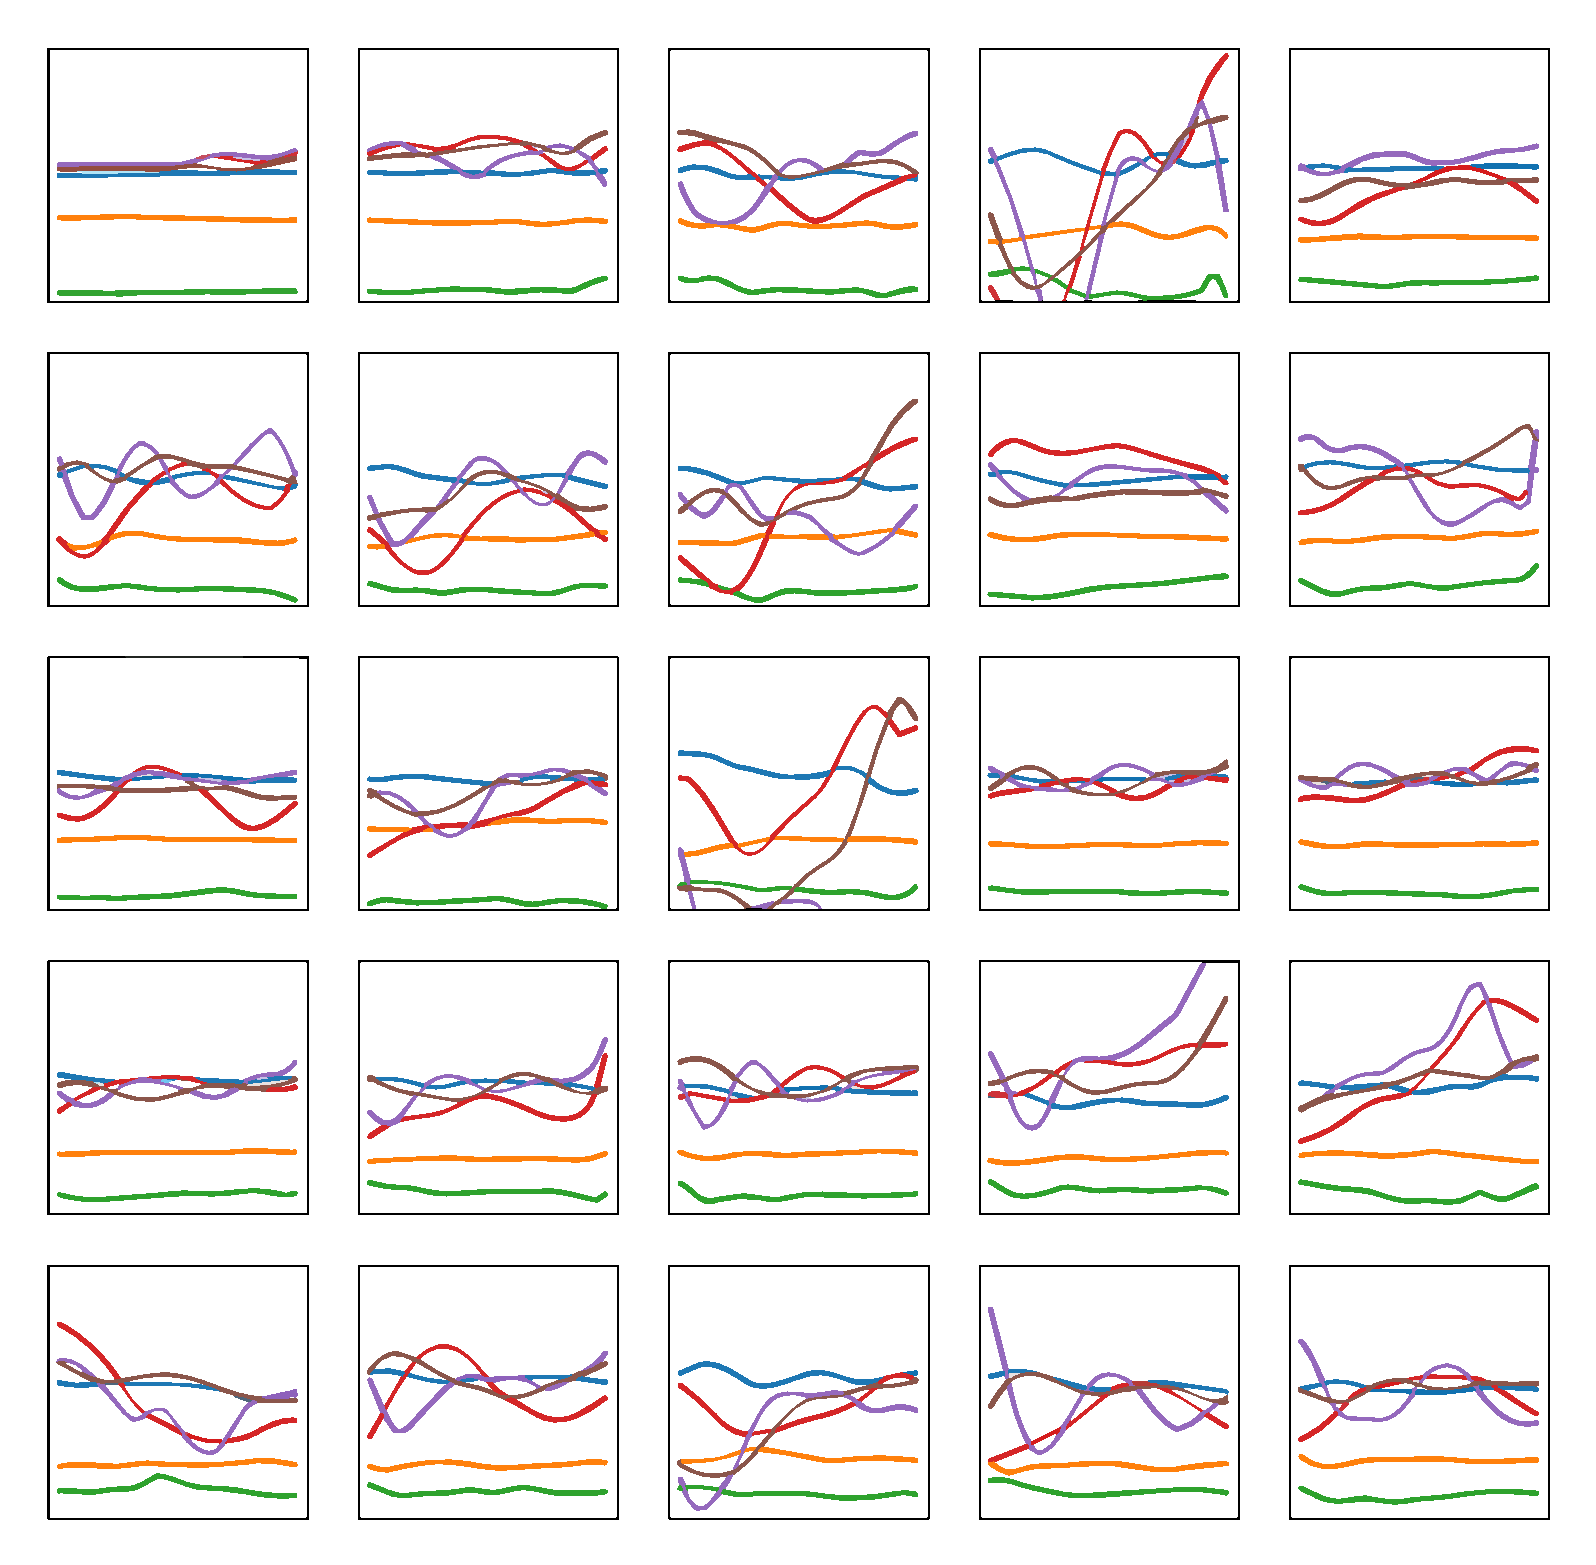
\includegraphics[width=\linewidth]{figures/side_channel_attack_results/sensor_data_non_touch_samples_received_at_GyroSec_server_without_Deceiver.pdf}
%     \caption{Non-touch samples without \framework{}}
%     \label{fig:dataSampleGyroSec_ntwoF}
% \end{subfigure}
% \hspace{0.9mm}
% \begin{subfigure}{0.4\linewidth}
%     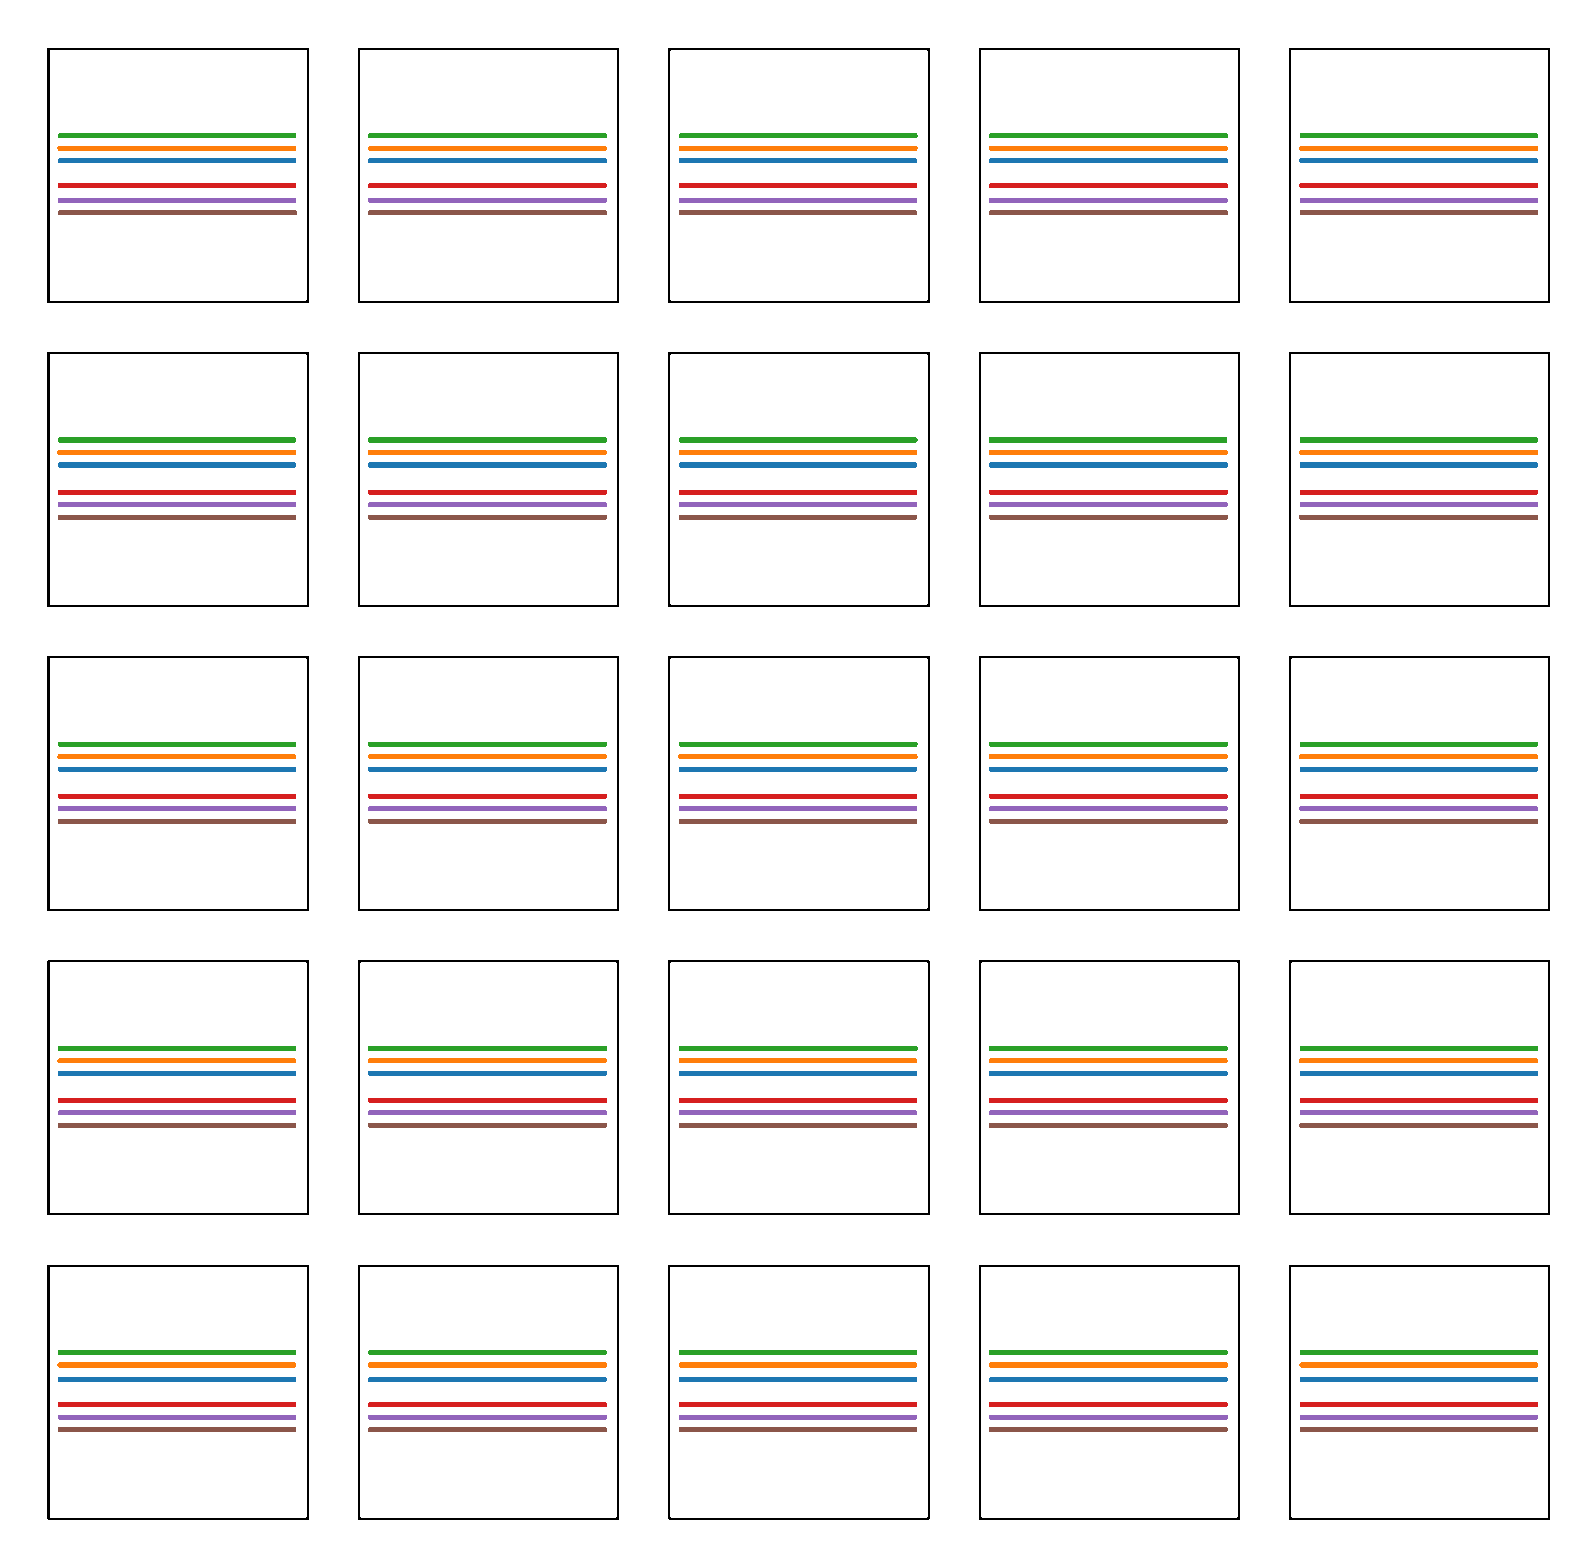
\includegraphics[width=\linewidth]{figures/side_channel_attack_results/sensor_data_non_touch_samples_received_at_GyroSec_server_with_Deceiver.pdf}
%     \caption{Non-touch samples with \framework{}}
%     \label{fig:dataSampleGyroSec_ntwF}
% \end{subfigure}
% \begin{subfigure}{0.4\linewidth}
%     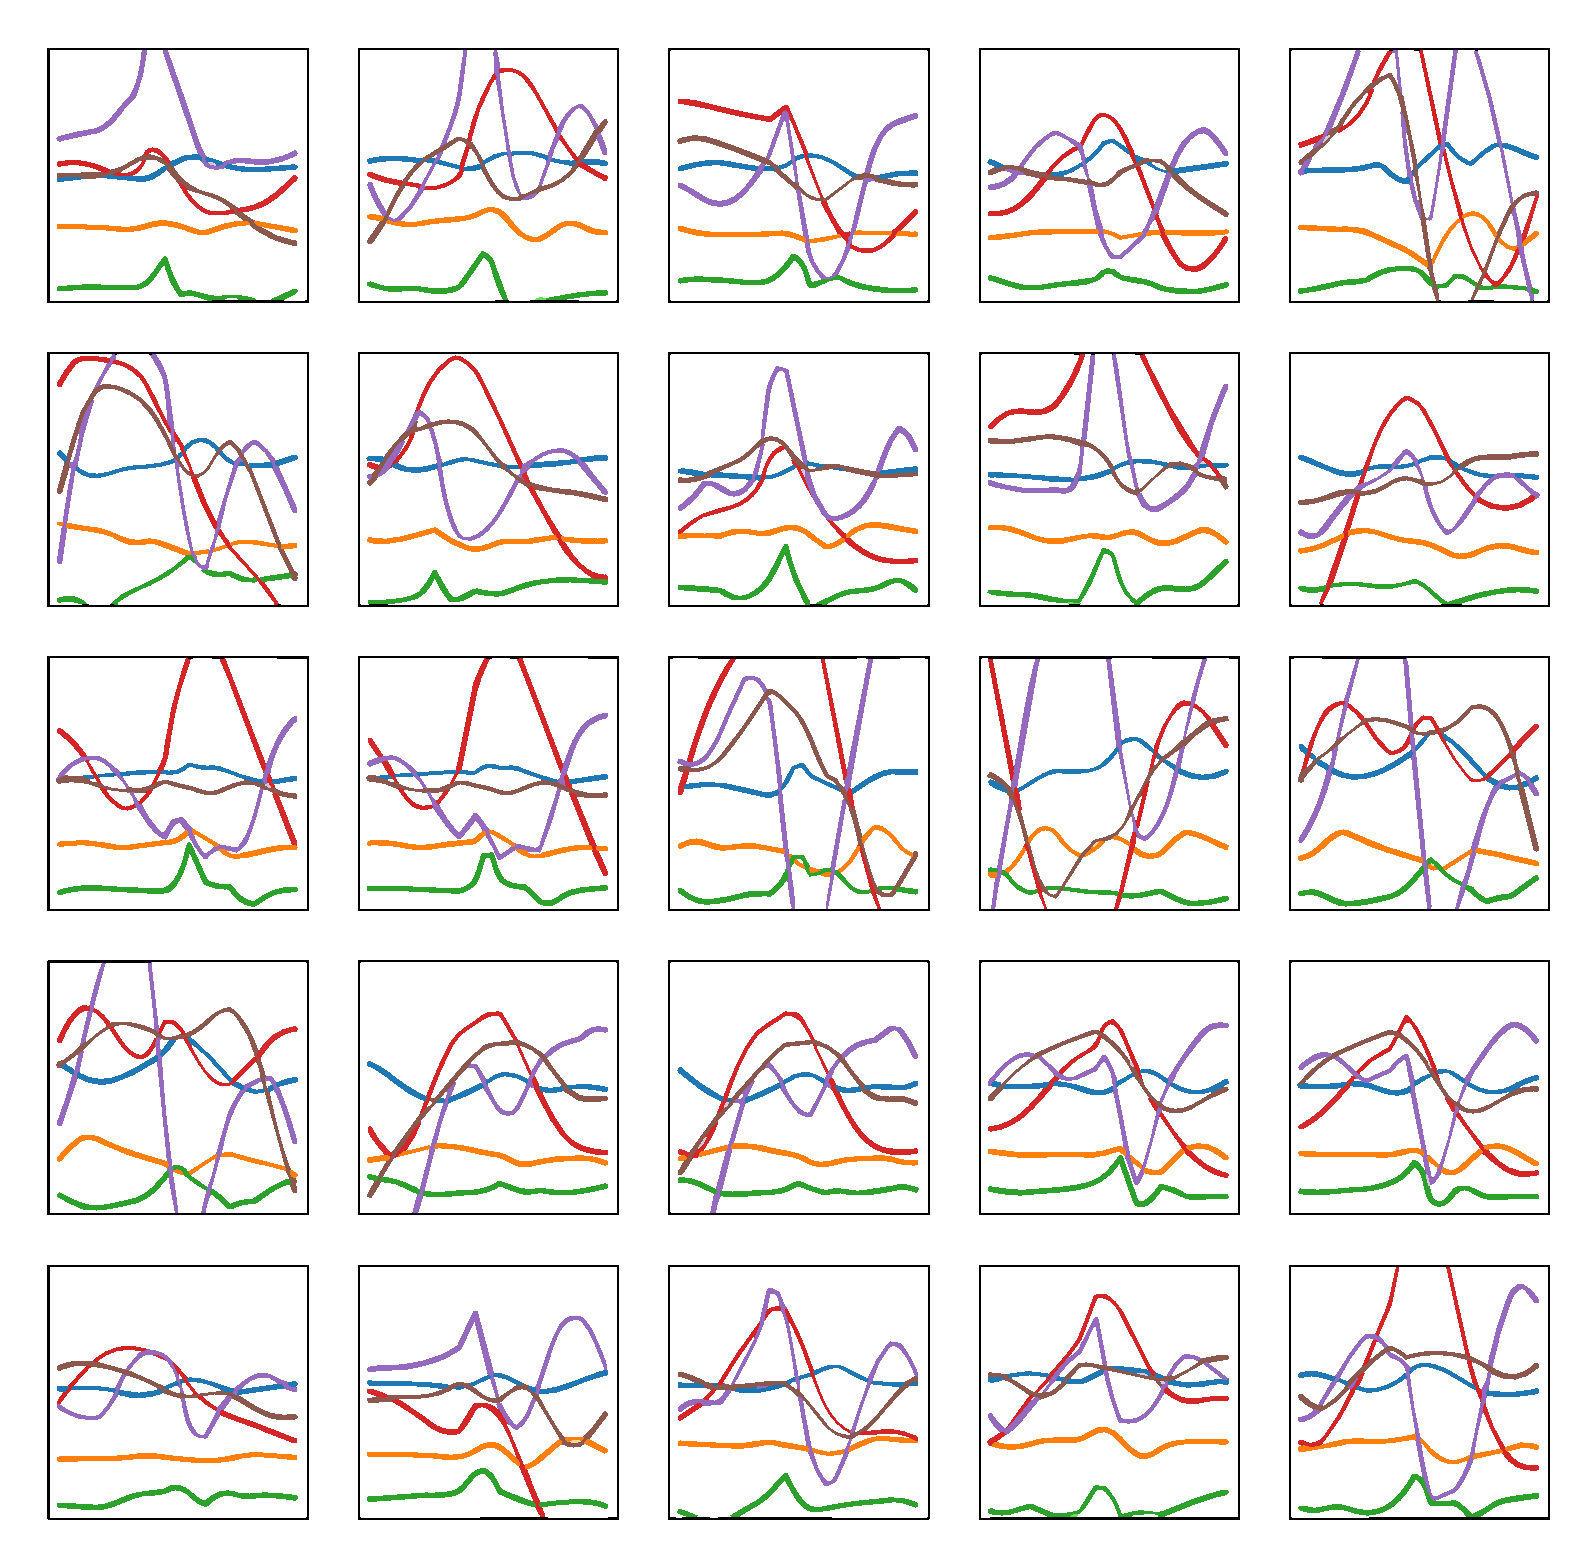
\includegraphics[width=\linewidth]{figures/side_channel_attack_results/sensor_data_touch_samples_received_at_GyroSec_server_without_Deceiver.pdf}
%     \caption{Touch samples without \framework{}}
%     \label{fig:dataSampleGyroSec_twoF}
% \end{subfigure}
% \hspace{0.9mm}
% \begin{subfigure}{0.4\linewidth}
%     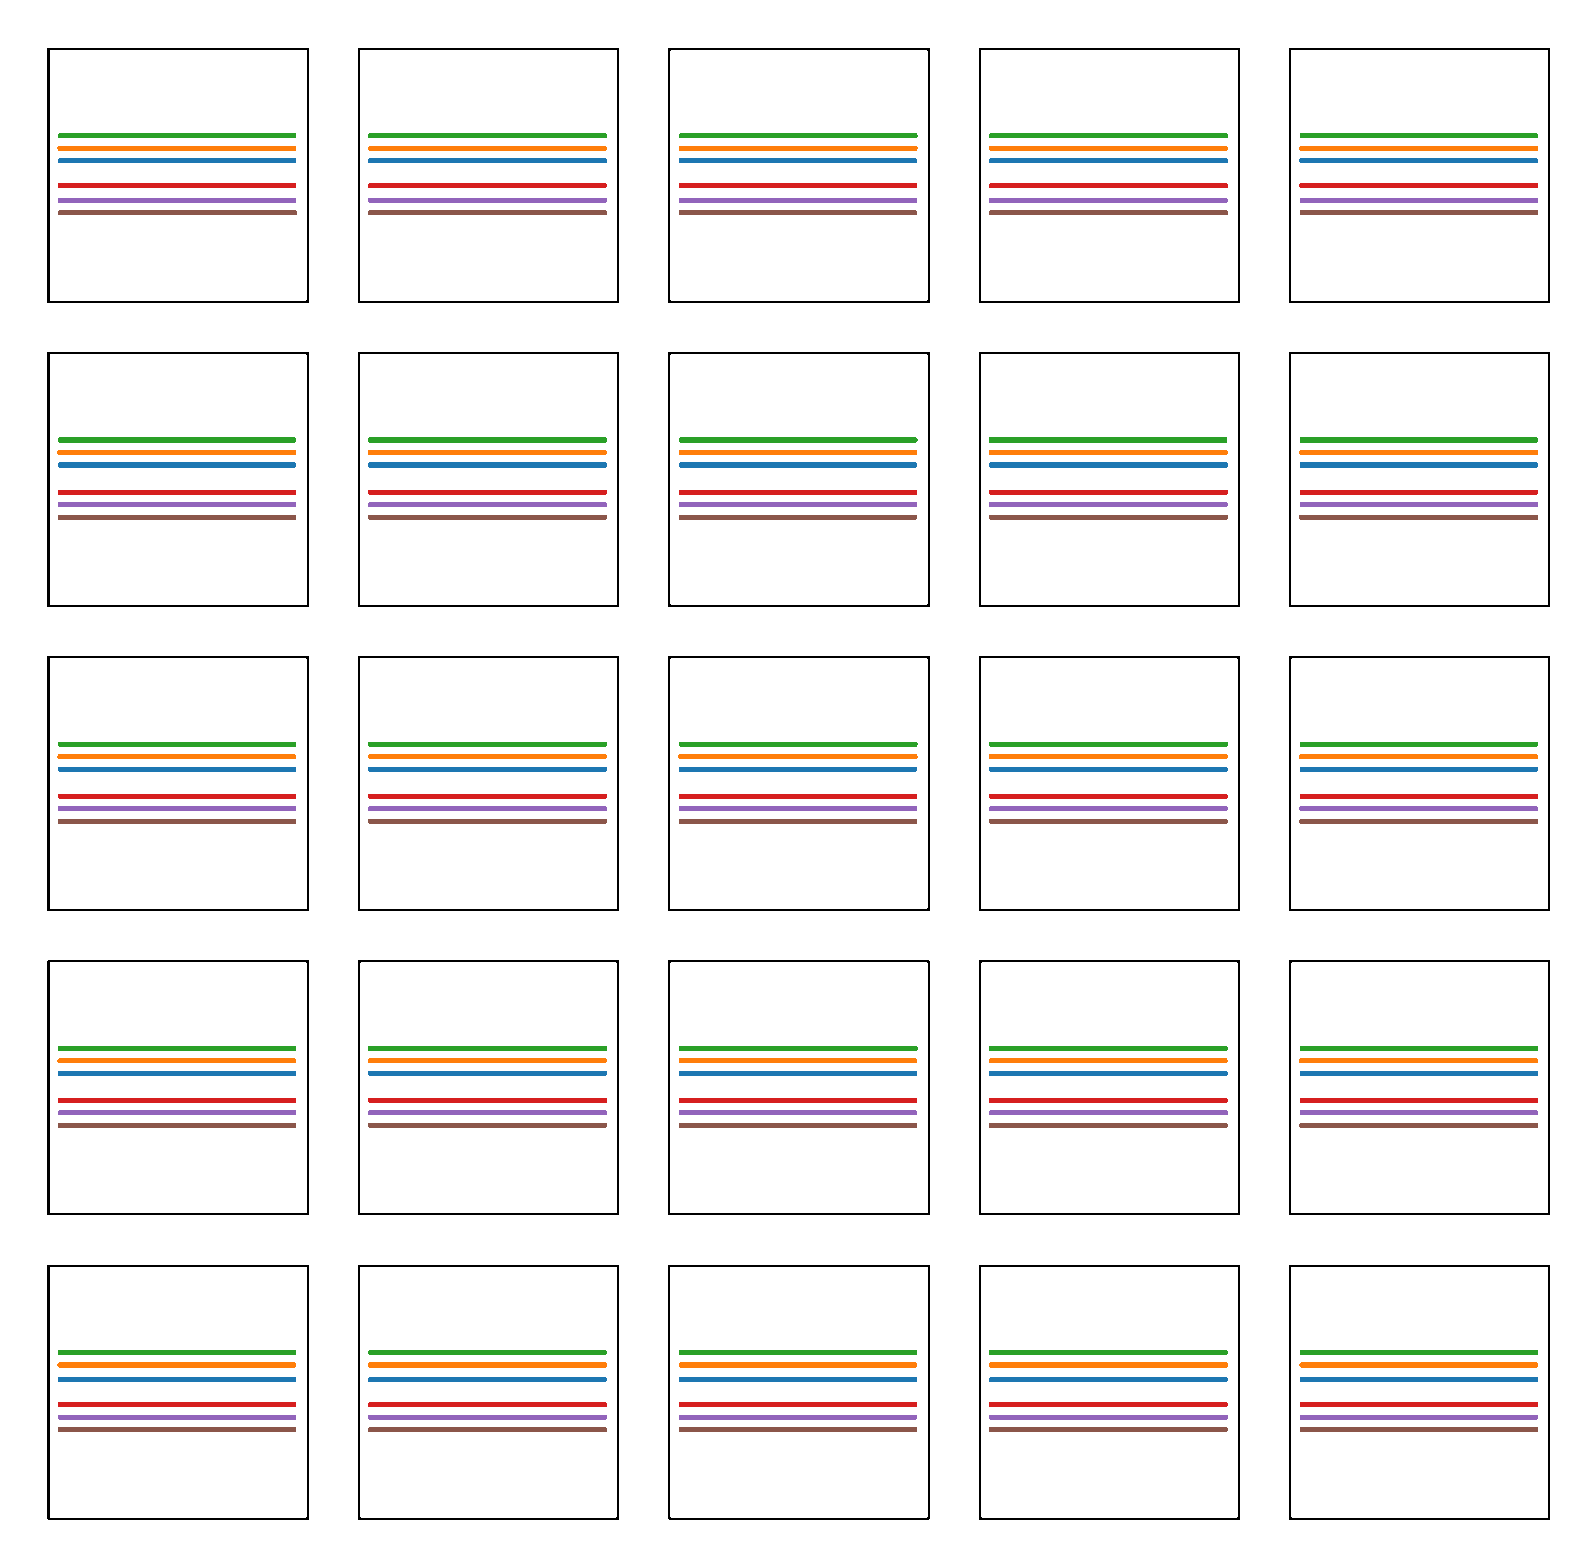
\includegraphics[width=\linewidth]{figures/side_channel_attack_results/sensor_data_touch_samples_received_at_GyroSec_server_with_Deceiver.pdf}
%     \caption{Touch samples with \framework{}}
%     \label{fig:dataSampleGyroSec_twF}
% \end{subfigure}
% \caption{Samples of Accelerometer and Gyroscope sensor data readings received at server.}
% \label{fig:dataSampleGyroSec}
% \end{figure}

%Nevertheless, our resolute experiments have demonstrated the defense mechanisms of the \framework{} against these side-channel attacks. 
By configuring \framework{} to deceive \textit{GyroSec}, we logged every instance of data access by \textit{GyroSec}, promptly notifying users of any background resource data breaches. \framework{} further deceived the data received by \textit{GyroSec}. Using the \textit{Policy Configurator} the accelerometer and gyroscope sensor readings were deceived as constant value for Gyrosec.
% It cleverly made the data harder to understand by using carefully chosen values set up in the \framework{}'s \textit{Policy Configurator}. As a result, \textit{GyroSec}'s server was rendered utterly impotent in its feeble attempts to predict touch positions, endowing users with unwavering privacy protection. 
Figure \ref{fig:tchPredict} illustrates reduction in \textit{GyroSec}'s ability to predict accurately by \framework{}. The prediction accuracy dropped from \textbf{81.22\%} to \textbf{5.36\%}, proving \framework{} to be a successful measure against Permission-based Side-Channel Attacks.

\begin{figure}[t]
\centering
\begin{subfigure}{0.35\linewidth}
    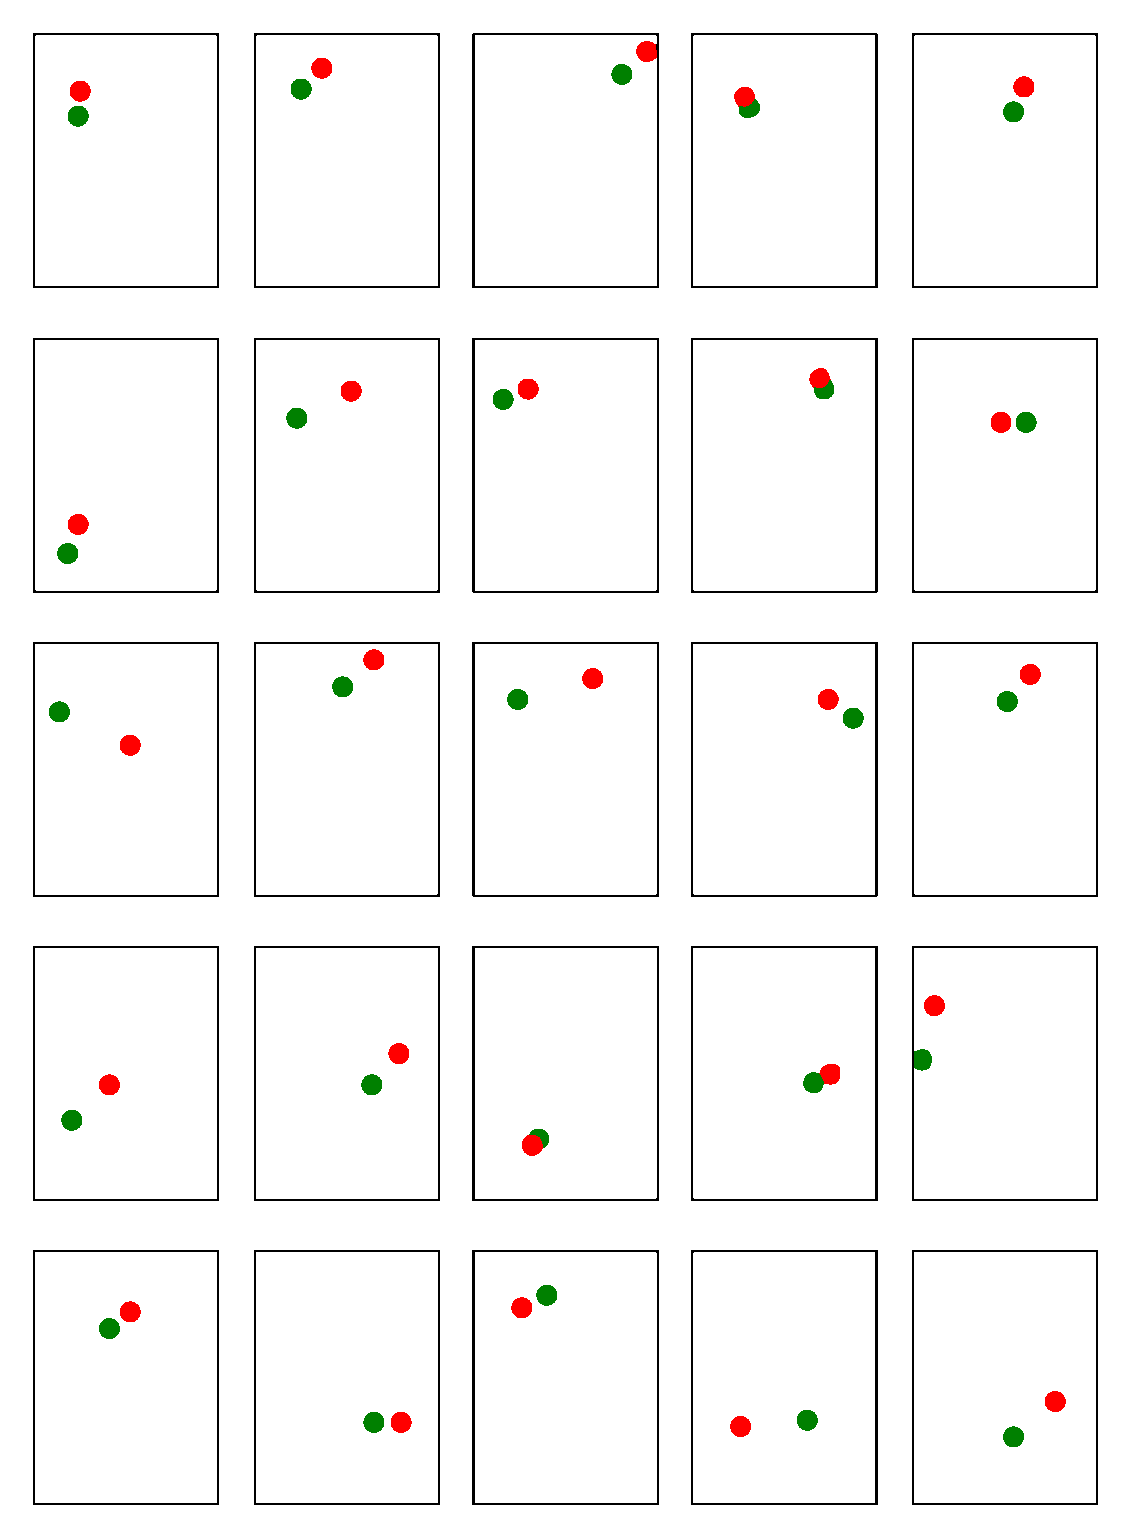
\includegraphics[width=\linewidth]{Figures/Side Channel Attacks/touch_prediction_samples_by_GyroSec_without_Deceiver.pdf}
    \caption{Without \framework{}}
    % \caption{Without \framework{} (High Accuracy achieved using true sensor readings)}
    \label{fig:tchPredict_wo_frmwrk}
\end{subfigure}
\hspace{0.9mm}
\begin{subfigure}{0.35\linewidth}
    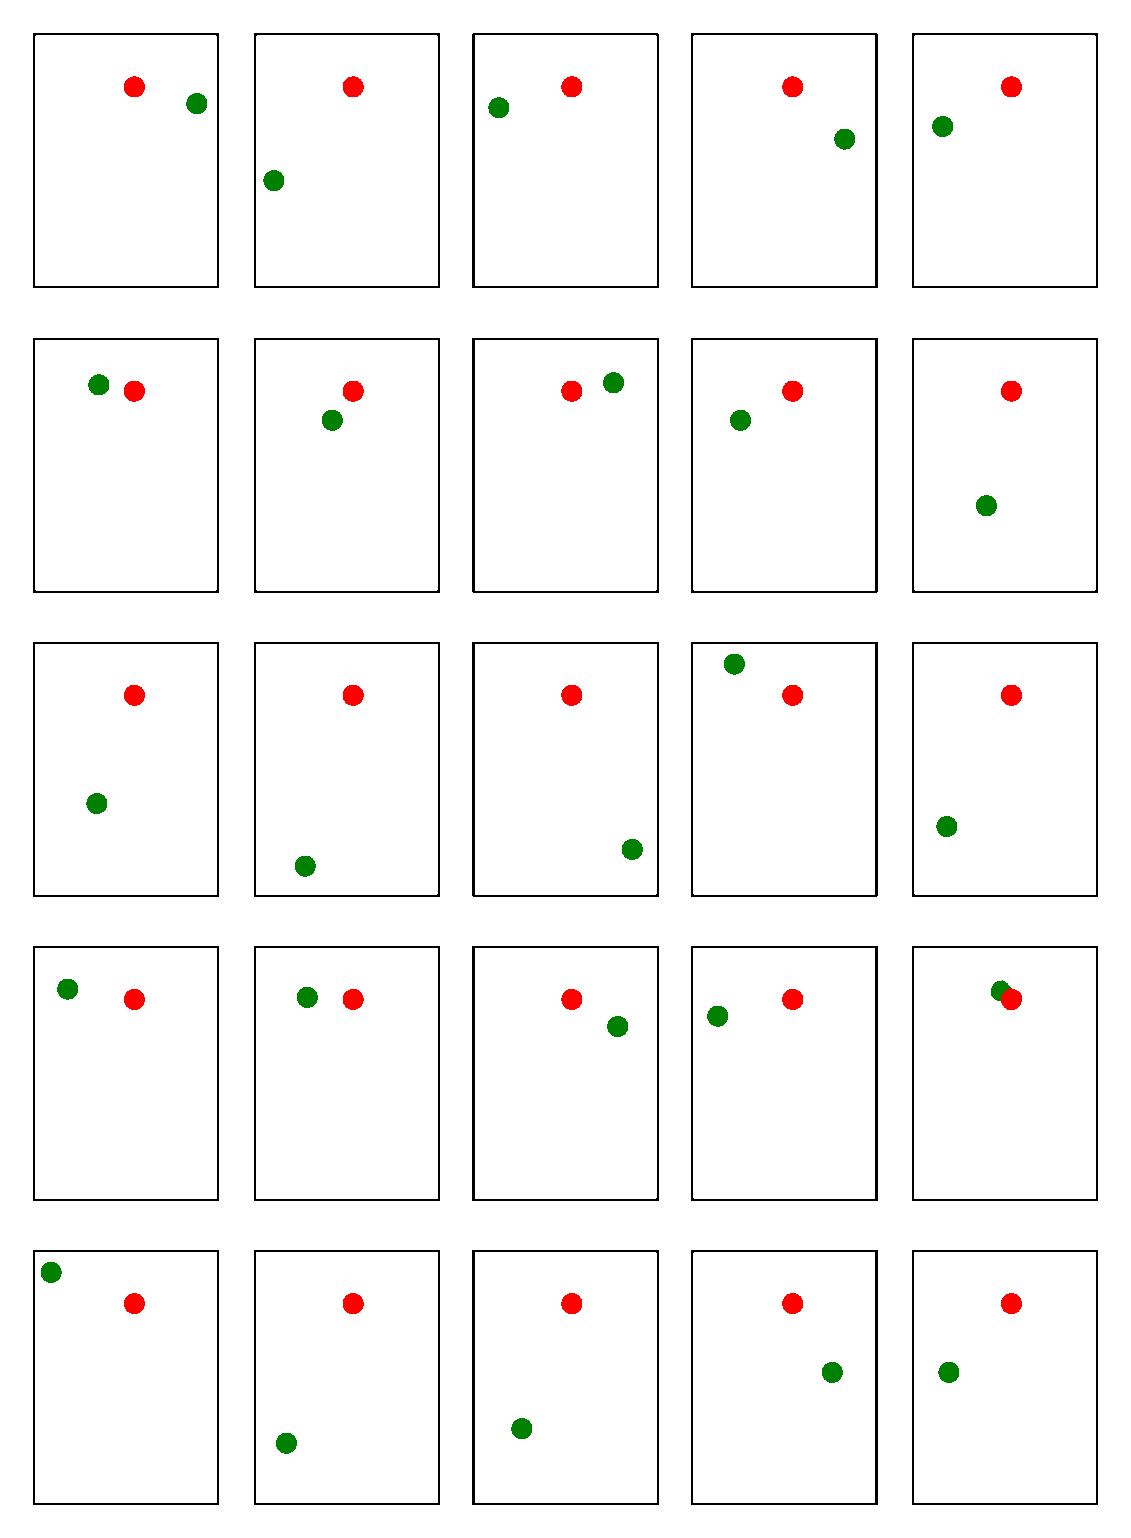
\includegraphics[width=\linewidth]{Figures/Side Channel Attacks/touch_prediction_samples_by_GyroSec_with_Deceiver.pdf}
    \caption{With \framework{}}
    \label{fig:tchPredict_w_frmwrk}
\end{subfigure}
\caption{Touch predicitions made by \textit{Gyrosec} server based on sensor readings received.}
\label{fig:tchPredict}
\end{figure}

%Hence, \framework{} counters Android side-channel attacks exploiting user data by manipulating the data the malicious app receives. The spoofed data compromises the integrity of the malicious server's results, rendering these attacks futile in gathering meaningful information about the user. 


\textit{Overall, this section shows that \framework could effectively stop most 
malicious behaviors giving better control to users over their sensitive data.}

% Based on the logs generated by \framework, we can confidently
% state that it effectively safeguards against malicious apps exploiting resource
% data for nefarious purposes.